
\newpage

\section{POS \& NER}

    \subsection{Part-of-Speech (POS) Tagging}
    
        Il \emph{Part-of-Speech tagging} assegna a ciascun token $w_i$ la sua categoria grammaticale $y_i$ (nome, verbo, aggettivo, ecc.), data la frase $w_{1:n}$. Formalmente è un problema di \textbf{sequence labeling}: vogliamo la sequenza di etichette più probabile
        
        \begin{wrapfigure}{r}{0.4\textwidth}
            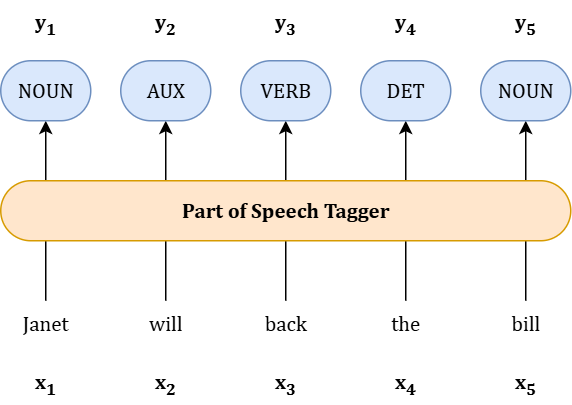
\includegraphics[width=1\linewidth]{imgs/schema_2_1.png}
            \label{fig:fig21}
        \end{wrapfigure}
        
        $$
        \hat{y}_{1:n} \;=\; \arg\max_{y_{1:n}} P\big(y_{1:n} \mid w_{1:n}\big)
        $$
        
        con vincoli di coerenza tra tag adiacenti (ad es. un determinante tende a precedere un nome) e dipendenza dal contesto.\\
        
        Il POS facilita l'analisi morfosintattica, la disambiguazione lessicale e step successivi (lemmatizzazione, parsing, NER). Un buon tagger riduce ambiguità come in: ``\textit{La porta è chiusa}'' (\textsc{porta}/NOUN) vs. ``\textit{Porta il libro}'' (\textsc{porta}/VERB), o ``\textit{banca}'' (istituto, NOUN) vs. ``\textit{banca a sinistra}'' (VERB colloquiale in alcuni registri), e gestisce clitici: ``\textit{gliel'ho detto}''.

        \subsubsection{Closed-Class vs. Open-Class Words}
        
            Nel lessico distinguiamo due famiglie con comportamento molto diverso: le \emph{parole chiuse} (\textit{closed class}) e le \emph{parole aperte} (\textit{open class}). La differenza non è solo tassonomica: influisce su frequenze, ambiguità, produttività morfologica e sulle strategie di tagging.
            
            \begin{itemize}
            
                \item Le \textbf{parole chiuse} appartengono a insiemi piccoli e relativamente stabili, con inventario quasi fisso nella lingua standard. Comprendono determinanti, preposizioni, congiunzioni, pronomi, ausiliari, particelle, negazioni, alcuni avverbi funzionali e la punteggiatura. Il loro ruolo è soprattutto \emph{grammaticale}: stabiliscono relazioni sintattiche e marcano funzioni.
                
                \item Le \textbf{parole aperte} formano classi a inventario non limitato e in continua crescita: nomi comuni e propri, verbi lessicali, aggettivi qualificativi, molti avverbi derivati e simboli tecnici. Il loro ruolo è \emph{lessicale/semantico}: introducono contenuto informativo e si arricchiscono con neologismi, prestiti, nomi propri.
                
            \end{itemize}
            
            Nel corpus, le parole chiuse sono altissime in frequenza ma poche come tipi distinti; contribuiscono alla testa della distribuzione (legge di Zipf). Le parole aperte hanno frequenza individuale più bassa e una \emph{coda lunga} di tipi rari; dominano la crescita del vocabolario secondo Heaps. Se $N$ è il numero di token e $|V|$ il vocabolario, la dinamica delle aperte segue spesso $|V_{\text{open}}(N)|\approx K\,N^{\beta}$ con $0<\beta<1$, mentre $|V_{\text{closed}}|$ rimane pressoché costante. La produttività morfologica è elevata nelle classi aperte (derivazione e flessione), mentre nelle chiuse è limitata o nulla.\\
            
            Per le classi chiuse il tagging sfrutta forti indizi lessicali: una tabella di frequenza parola\,$\to$\,tag è spesso sufficiente e l’ambiguità è bassa (ad es. \emph{di} è quasi sempre \textsc{ADP}). Per le classi aperte l’ambiguità è alta (\emph{porta} NOUN/VERB) e la disambiguazione richiede contesto sintagmatico e morfologia. Inoltre, gli OOV nascono prevalentemente nelle classi aperte; per questo gli embedding subword e la gestione di suffissi/prefissi aiutano soprattutto su nomi, verbi e aggettivi.

        \newpage
        
        Adottiamo le classi \textbf{Universal Dependencies (UPOS)}:         
        
        \begin{center}
            \begin{tabular}{llll}
            \toprule
            & \textbf{Tag} & \textbf{Descrizione} & \textbf{Esempio IT} \\
            \midrule
            \textbf{Open Class} & ADJ & aggettivo & \emph{nuovo}, \emph{bello} \\
            & ADV & avverbio & \emph{molto}, \emph{sempre} \\
            & NOUN & nome comune & \emph{porta}, \emph{libro} \\
            & VERB & verbo lessicale & \emph{portare}, \emph{studiare} \\
            & PROPN & nome proprio & \emph{Roma}, \emph{San\_Francesco} \\
            & INTJ & interiezione & \emph{oh}, \emph{eh} \\
            \midrule
            \textbf{Closed Class} & ADP & preposizione & \emph{di}, \emph{a}, \emph{con} \\
            & AUX & ausiliare & \emph{essere}, \emph{avere} (aus.) \\
            & CCONJ & congiunzione coord. & \emph{e}, \emph{ma}, \emph{o} \\
            & DET & determinante & \emph{il}, \emph{una}, \emph{questo} \\
            & NUM & numero & \emph{due}, \emph{100} \\
            & PART & particella & \emph{non}, \emph{ci} (part.) \\
            & PRON & pronome & \emph{io}, \emph{gli}, \emph{che} \\
            & SCONJ & congiunzione sott. & \emph{che}, \emph{perché} \\
            \midrule
            \textbf{Other} & PUNCT & punteggiatura & \emph{,} \emph{.} \emph{—} \\
            & SYM & simbolo & \emph{€}, \emph{\%} \\
            & X & altro & stringhe miste, codice \\
            \bottomrule
            \end{tabular}
        \end{center}

        La grana fine (morfologia: genere/numero, tempo/modo/persona) si esprime con feat addizionali e talvolta con un tagset più dettagliato (\emph{XPOS}) quando serve compatibilità con risorse legacy.\\
        
        Molte forme sono \emph{ambigue} (es. ``porta'' NOUN/VERB). La disambiguazione sfrutta il contesto: $P(y_i\mid y_{i-1},w_{1:n})$ differisce se il token precedente è un determinante, un pronome o una preposizione. Decisioni di pre-processing influenzano il tagging: separare "l'" da \emph{ho} aiuta a assegnare \textsc{DET} e \textsc{AUX} corretti; trattare MWE come \emph{New\_York} evita confondere \textsc{PROPN} con due token separati.\\
        
        La metrica standard è l'\textbf{accuracy} per token:
        
        $$
        \mathrm{Acc} \;=\; \frac{\#\,\text{token con tag corretto}}{\#\,\text{token totali}}
        $$
        
        Con etichette esclusive per token, l'accuracy coincide con la micro-$F_1$. È buona prassi riportare anche errori per classe (confusioni tipiche: \textsc{AUX}/\textsc{VERB}, \textsc{ADJ}/\textsc{NOUN}) e analizzare le prestazioni su \emph{OOV} e domini diversi (news vs. social). Errori di tokenizzazione o di normalizzazione propagano a valle e vanno contabilizzati.\\

        Su corpora bilanciati e ben tokenizzati, i tagger neurali moderni in italiano e lingue europee raggiungono tipicamente $\mathrm{Acc} \ge 97\%$ con encoder pre-addestrati; CRF e HMM di buona qualità si collocano poco sotto. In domini rumorosi o con forte variazione morfologica l'accuracy cala sensibilmente: la gestione di OOV, clitici e varianti ortografiche incide molto.

    \newpage

    \subsection{Named Entity Recognition (NER)}
    
        La \emph{Named Entity Recognition} identifica e classifica menzioni di entità nel testo (persone, organizzazioni, luoghi, date, quantità, ecc.). Data una sequenza di token $w_{1:n}$, l’obiettivo è produrre una sequenza di etichette $y_{1:n}$ che segmenti le menzioni e ne assegni il tipo. È un problema di \textbf{sequence labeling} con vincoli strutturali sui confini e sulla coerenza delle etichette.\\
        
        Si rappresentano le menzioni come segmenti contigui con schemi standard:
        
        \begin{itemize}
        
            \item \textbf{BIO}: \texttt{B-}\emph{TYPE} (inizio), \texttt{I-}\emph{TYPE} (interno), \texttt{O} (fuori da entità).
          
            \item \textbf{BIOES}: aggiunge \texttt{E-}\emph{TYPE} (fine) e \texttt{S-}\emph{TYPE} (menzione di un solo token) per rendere più espliciti i confini.
            
        \end{itemize}
        
        \paragraph{Ex.\\}

        \begin{center}
            \begin{tabular}{l l l l}
                \hline
                \textbf{Words} & \textbf{IO Label} & \textbf{BIO Label} & \textbf{BIOES Label} \\
                \hline
                Jane       & I-PER & B-PER & B-PER \\
                Villanueva & I-PER & I-PER & E-PER \\
                of         & O     & O     & O     \\
                United     & I-ORG & B-ORG & B-ORG \\
                Airlines   & I-ORG & I-ORG & I-ORG \\
                Holding    & I-ORG & I-ORG & E-ORG \\
                discussed  & O     & O     & O     \\
                the        & O     & O     & O     \\
                Chicago    & I-LOC & B-LOC & S-LOC \\
                route      & O     & O     & O     \\
                .          & O     & O     & O     \\
                \hline
            \end{tabular} 
        \end{center}       
        
        La metrica standard valuta \emph{menzioni complete} (span + tipo). Si computano precision, recall e $F_1$ su insiemi di menzioni predette ($\widehat{\mathcal{E}}$) e gold ($\mathcal{E}$):
        
        $$
            \mathrm{Prec}=\frac{|\widehat{\mathcal{E}}\cap\mathcal{E}|}{|\widehat{\mathcal{E}}|},\qquad
            \mathrm{Rec}=\frac{|\widehat{\mathcal{E}}\cap\mathcal{E}|}{|\mathcal{E}|},\qquad            
            \mathrm{F}_1=\frac{2\,\mathrm{Prec}\cdot\mathrm{Rec}}{\mathrm{Prec}+\mathrm{Rec}}
        $$
        
        Un match è corretto se \emph{entrambi} i confini e il tipo coincidono. È buona prassi riportare anche i risultati per classe (PER/ORG/LOC/\dots) e distinguere micro e macro-averaging.\\
        
        Tokenizzazione e normalizzazione coerenti sono cruciali: menzioni composte (\textit{San Francesco}), apostrofi e accenti influiscono sui confini. Le \textbf{gazetteer} (liste di nomi propri, toponimi, sigle) sono utili come feature ma vanno gestite con cura per evitare overfitting di dominio. La rappresentazione a caratteri/subword mitiga gli OOV e cattura regolarità ortografiche (suffissi aziendali, notazioni alfanumeriche).\\
        
        Nomi comuni vs. propri (\textit{apple} vs. \textit{Apple}), metonimie (\textit{Roma} città vs. squadra), entità annidate o sovrapposte (\textit{Università di [B-ORG Roma [I-LOC Tre]]}), e sigle creative richiedono bias di decodifica e/o schemi di annotazione dedicati (NER piatto vs. NER annidato). In corpora standard, le menzioni sono \emph{non sovrapposte} e il modello produce una sola etichetta per token.\\
        
        Su corpora ben bilanciati e in lingua standard, modelli neurali con encoder pre-addestrati e CRF raggiungono spesso $\mathrm{F}_1$ \,$\ge$\,$90\%$ a livello di entità per classi frequenti (PER/ORG/LOC). Il calo è più marcato su classi rare (MISC, eventi) o in domini rumorosi (social, OCR). Errori tipici: confini sballati di un token (\texttt{B-}/\texttt{E-}), tipo corretto ma span errato, o tipo confuso tra ORG/LOC per toponimi istituzionali.

    \newpage

    \subsection{Standard Algorithms for NER/POS Tagging}

        Dato un input $w_{1:n}$ (token), vogliamo la sequenza di etichette $y_{1:n}$ che massimizza la probabilità condizionata o congiunta a seconda del modello:
        
        $$
            \hat y_{1:n}=\arg\max_{y_{1:n}} P(y_{1:n}\mid w_{1:n})\quad\text{(discriminativo)}\qquad\text{o}\qquad \hat y_{1:n}=\arg\max_{y_{1:n}} P(y_{1:n},w_{1:n})\quad\text{(generativo)}.
        $$
        
        Alcune famiglie di modelli supervisionati per l'etichettatura di sequenza sono
    
            \subsubsection{Hidden Markov Models}
            
                \begin{wrapfigure}{r}{0.35\textwidth}
                    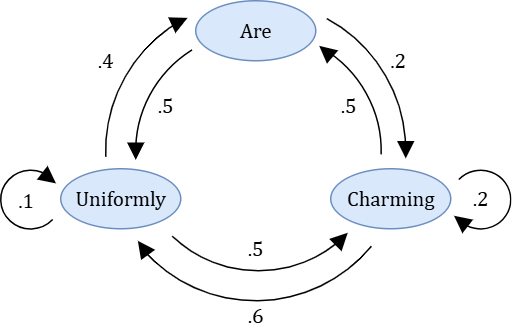
\includegraphics[width=1\linewidth]{imgs/schema_2_2.png}
                    \label{fig:fig22}
                \end{wrapfigure}    
                Un \textbf{HMM} è un modello generativo per l'etichettatura di sequenza. Assume una catena di stati latenti $y_{1:n}$ (i tag) che genera i token osservati $w_{1:n}$ con emissioni condizionate dallo stato corrente.
                
                \begin{itemize}
                
                    \item transizioni tra tag $a_{y'\!,y}=P(y_i{=}y\mid y_{i-1}{=}y')$;
                    
                    \item emissioni $b_y(w)=P(w_i{=}w\mid y_i{=}y)$.
                    
                \end{itemize}
                
                La congiunta fattorizza come
    
                $$
                    P(y_{1:n}, w_{1:n}) \;=\; \pi_{y_1}\, b_{y_1}(w_1)\, \prod_{i=2}^{n} a_{y_{i-1},y_i}\, b_{y_i}(w_i).
                $$\\
                In pratica si aggiungono stati speciali $\langle s\rangle$ e $\langle/ s\rangle$ per inizio/fine frase. 
                
                \paragraph{Codifica di Viterbi.} 
                \begin{wrapfigure}{r}{0.35\textwidth}
                    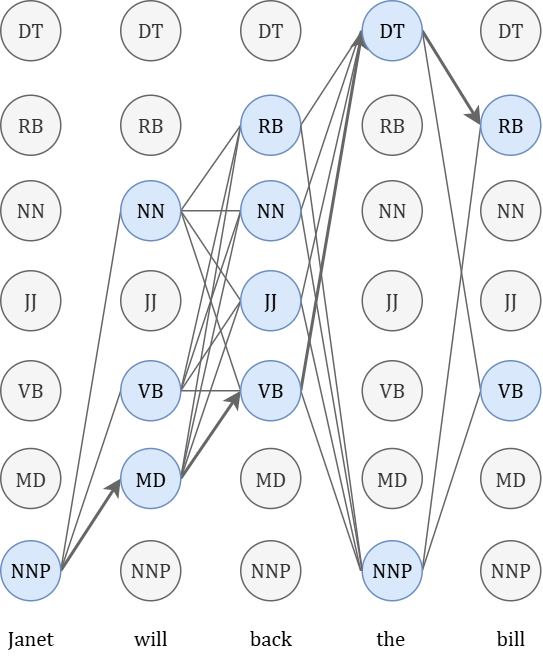
\includegraphics[width=1\linewidth]{imgs/schema_2_3.png}
                    \label{fig:fig23}
                \end{wrapfigure}
                Dato $w_{1:n}$, cerchiamo la sequenza di tag a massima verosimiglianza \emph{a posteriori} (MAP):
                
                \begin{gather}
                    \notag\hat y_{1:n} \,=\, \arg\max_{y_{1:n}} P(y_{1:n} \mid w_{1:n}) \;=\; \arg\max_{y_{1:n}} P(y_{1:n}, w_{1:n}).
                \end{gather}
                
                La cui \textbf{ricorrenza di Viterbi} in log-spazio è
                
                
                \begin{gather}
                    \notag\delta_i(y) \;=\; \max_{y'}\Big\{\, \delta_{i-1}(y') + \log a_{y'\!,y} \Big\} + \log b_y(w_i),\\[2ex]
                    \notag\delta_1(y)=\log \pi_y + \log b_y(w_1),
                \end{gather}
                
                con backpointer $\psi_i(y)=\arg\max_{y'}\{\delta_{i-1}(y') + \log a_{y'\!,y}\}$ e ricostruzione all’indietro a partire da $\hat y_n=\arg\max_y \delta_n(y)$.
                
                \paragraph{Addestramento supervisionato (MLE).}
                Con training etichettato, le stime di massima verosimiglianza sono basate sui conteggi:
                
                $$
                    \hat \pi_y = \frac{c(y\text{ in posizione 1})}{\sum_{y'} c(y' \text{ in posizione 1})},\quad
                    \hat a_{y'\!,y} = \frac{c(y'\!\to y)}{\sum_{y''} c(y'\!\to y'')},\quad
                    \hat b_y(w) = \frac{c_y(w)}{\sum_{w'} c_y(w')},
                $$\\                
                con $c(y'\!\to y)$ conteggi di transizioni adiacenti nel corpus e $c_y(w)$ conteggi di emissione della parola $w$ dal tag $y$.\\
                
                In POS l’emissione è tipicamente parola\,$\to$\,tag; in NER si può applicare alle etichette BIO/BIOES. Gli HMM sono competitivi come baseline, specialmente con pochi dati, e beneficiano molto di: (i) tokenizzazione coerente, (ii) gestione di MWE per nomi propri, (iii) smoothing mirato sulle emissioni (classe aperta) e dizionari per le classi chiuse.
    
            \subsubsection{Conditional Random Fields (CRF)}
            
                Un \textbf{CRF a catena lineare} modella direttamente la probabilità condizionata di una sequenza di etichette $y_{1:n}$ dato l’input $x_{1:n}$ (token, più eventuali feature), combinando molteplici indizi locali in modo \emph{globale} sull’intera frase.\\
                
                Sia $\phi_k(y_{i-1},y_i,x,i)$ una funzione di feature locale (di solito binaria: $1$ se la regola vale, $0$ altrimenti) che dipende solo dalla \textit{coppia di tag adiacenti} $(y_{i-1},y_i)$, \textit{dalla posizione} $i$ e \textit{dall’input della frase} $x$. Con pesi $\theta_k$, la probabilità è
                
                $$
                    P_\theta(y\mid x) 
                    \;=\; \frac{1}{Z_\theta(x)} \; \exp\!\Bigg(\sum_{i=1}^{n} \sum_{k} \theta_k\, \phi_k(y_{i-1},y_i,x,i)\Bigg),
                $$
                
                con partizione (\emph{normalizzatore})
                
                $$
                    Z_\theta(x) \,=\, \sum_{y'\in\mathcal{Y}^n} \exp\!\Bigg(\sum_{i=1}^{n} \sum_{k} \theta_k\, \phi_k(y'_{i-1},y'_i,x,i)\Bigg).
                $$
                
                \textbf{\textit{Nota}}: $Z_\theta(x)$ dipende solo da $x$ e $\theta$, quindi non influisce sull’$\arg\max_y$ in decodifica.\\
                
                Convenientemente si raggruppano le feature in \emph{potenziali} di transizione e di stato: 
                
                $$
                    \mathrm{score}(y\mid x) \,=\, \sum_{i=1}^{n} \big( \, s_i(y_i,x) + t_i(y_{i-1},y_i,x) \,\big),
                $$
                
                con $s_i$ funzioni sul tag corrente e $t_i$ funzioni sulla coppia $(y_{i-1},y_i)$. Allora $P_\theta(y\mid x) \propto \exp(\mathrm{score}(y\mid x))$.
                
                \paragraph{Decodifica di Viterbi.}
                La sequenza più probabile si ottiene massimizzando la somma degli score:
                
                $$
                    \hat y_{1:n} \,=\, \arg\max_{y\in\mathcal{Y}^n} \sum_{i=1}^{n} \big( s_i(y_i,x) + t_i(y_{i-1},y_i,x) \big),
                $$
                
                che si risolve con \textbf{Viterbi} usando come emissioni/transizioni i punteggi $s_i$ e $t_i$ calcolati dalle feature del CRF.
                
                \paragraph{Addestramento Supervisionato(MLE).}
                Dato un dataset annotato $\{(x^{(j)},y^{(j)})\}_{j=1}^M$, si massimizza la log-verosimiglianza regolarizzata
                
                $$
                    \mathcal{L}(\theta) \,=\, \sum_{j=1}^{M} \Big[\, \sum_{i,k} \theta_k\,\phi_k(y^{(j)}_{i-1},y^{(j)}_{i},x^{(j)},i) \,-\, \log Z_\theta(x^{(j)}) \,\Big] \; - \; \frac{\lambda}{2}\,\lVert\theta\rVert_2^2.
                $$
                
                Il gradiente è la differenza tra \emph{conteggi empirici} e \emph{conteggi attesi sotto il modello}:
                
                $$
                    \frac{\partial \mathcal{L}}{\partial \theta_k} \,=\, \sum_{j,i} \phi_k\big(y^{(j)}_{i-1},y^{(j)}_{i},x^{(j)},i\big) \; - \; \sum_{j} \sum_{y} P_\theta(y\mid x^{(j)})\, \sum_{i} \phi_k(y_{i-1},y_i,x^{(j)},i).
                $$
                
                I termini attesi si calcolano in $\mathcal{O}(n\,|\mathcal{Y}|^2)$ con \textbf{forward–backward}. In pratica si usa ottimizzazione numerica (SGD/Adam, L-BFGS) con \emph{cross-entropy} e regolarizzazione.

                \newpage
                
                Le feature locali sono indicatori binari costruiti da \textbf{template} astratti riempiti dai valori osservati. Esempi tipici per POS/NER:
                
                \begin{itemize}
                
                    \item \textbf{Lessico/forma}: parola, minuscola/maiuscola, cifre, punteggiatura, \emph{wordshape} (p.es. \texttt{Xx\_xx}, \texttt{xx\d}).
                    
                    \item \textbf{Contesto}: token a \,$\pm1$, \,$\pm2$ posizioni; bigrammi di tag $(y_{i-1},y_i)$.
                    
                    \item \textbf{Morfologia}: prefissi/suffissi di lunghezza 1–4; segnalazione di apostrofi/clitici.
                    
                    \item \textbf{Gazetteer}: appartenenza a liste (toponimi, organizzazioni), con attenzione all’overfitting di dominio.
                    
                    \item \textbf{Vincoli BIO/BIOES} (per NER): proibizioni di transizioni illegali (es. \texttt{I-LOC} non può seguire \texttt{O}).
                    
                \end{itemize}
                
                Tutte possono essere codificate come binarie; feature numeriche si includono come valori reali.\\
                
                A differenza di un softmax token-wise (MaxEnt), il CRF \emph{normalizza globalmente} sulla sequenza, modellando dipendenze tra tag adiacenti e riducendo incoerenze (es. sequenze BIO impossibili). Rispetto a HMM, consente \emph{feature arbitrarie} sull’osservazione senza dover espandere lo spazio degli stati.\\                

            \noindent\newline
            Oltre alle due di modelli appena descritte, abbiamo inoltre
    
            \begin{itemize}
    
                \item\textbf{Neural sequence models (RNN/BiLSTM/Transformer)}: Qui le rappresentazioni si imparano dai dati. Si usano embedding a parola/subword e un codificatore contestuale, ad esempio
                
                $$
                    \mathbf{h}_{1:n}=\mathrm{BiLSTM}(\mathrm{emb}(w_{1:n}))\quad\text{oppure}\quad \mathbf{H}=\mathrm{Transformer}(w_{1:n}),
                $$
                
                seguiti da uno strato di classificazione token-wise (softmax) o un CRF in uscita per decodifica strutturata. Con encoder pre-addestrati, questi modelli riducono la necessità di feature manuali e gestiscono bene OOV e variazioni di dominio.
                
                \item\textbf{Large Language Models (LLM) fine-tunati}: Encoder pre-addestrati (es. BERT e varianti) si usano come backbone e si fine-tunano per POS/NER con una testa di classificazione (spesso con CRF). Il fine-tuning su un set annotato fornisce prestazioni allo stato dell'arte con minima ingegneria delle feature.
            
            \end{itemize}
            
            Tutti i modelli richiedono un \textbf{training set etichettato a mano} e sfruttano le stesse fonti informative: nei modelli "classici" tramite \emph{feature umane} (morfologia, maiuscole, liste), nei modelli neurali tramite \emph{representation learning}. Su inglese standard, a parità di dati e pre-processing, le prestazioni sono \emph{simili} (POS \(\approx 97\%\) di accuracy; NER con $F_1$ elevati sulle classi frequenti), con differenze dovute soprattutto a dominio, tokenizzazione e gestione di OOV.\\
            
            La scelta del miglior modello può dipendere da vari fattori:\newline
            \emph{Pochi dati o necessità di vincoli strutturali espliciti}: CRF (magari con livello a caratteri) è una scelta robusta.\newline
            \emph{Dati moderati/ampi o dominio eterogeneo}: modelli neurali con encoder pre-addestrato (BiLSTM/Transformer) e, se serve, CRF in uscita.\newline
            \emph{Baseline/risorse minime}: HMM fornisce una base semplice e riproducibile.
     
            